\subsubsection{Comunicación con central operativa}

La comunicación del SAL/T con la central operativa se va a realizar a través del módulo ESP32 que permite la conectividad Wi-Fi utilizando el protocolo MQTT para el intercambio de mensajes. \\

El módulo ESP32 se conecta al MCU utilizando la interfaz UART4 con una configuración 8N1 con un \textit{baudrate} de 115.200 y sobremuestreo de 16 veces. Esta comunicación va a ser de manera bidireccional, ya que ambos dispositivos van a transmitir y recibir datos. El ESP32 está configurado para hacer principalmente de puente entre el MCU y el broker MQTT; esto significa que cualquier mensaje que reciba del MCU, lo va a retransmitir al MQTT y cualquier mensaje que recibe de MQTT lo va a retransmitir al MCU. También tiene la funcionalidad de mantener la fecha y hora del SAL/T actualizado ante un eventual corte en la alimentación consultando un cliente NTP (Network Time Protocol) para obtener la hora actual de un servidor en Internet.\\ 

El ESP32 permite la configuración de los datos de hasta dos redes Wi-Fi y constantemente va a estar verificando la conexión y, en caso de desconexión, intentando conectarse de manera alternada a cualquiera de ellas. Una vez conectado a una red Wi-Fi, se va a registrar en el broker MQTT configurado donde va a suscribir al \textit{topic} salt\_remote\_command. En este \textit{topic}, la central operativa va a publicar los comandos a aplicar sobre el SAL/T por lo que cualquier mensaje recibido va a ser enviado al MCU para su procesamiento. Además, cada 10 segundos el módulo va a consultar el servidor NTP pool.ntp.org \cite{ntp} para obtener la fecha y hora exacta y transmitírsela al SAL/T. \\ 

En sentido inverso, el ESP32 está constantemente levantando cualquier mensaje que pueda recibir por la interfaz UART. Al recibir un mensaje (terminado por un retorno de línea), el módulo va a leer los primeros caracteres (contando hasta un carácter delimitador) para determinar a qué \textit{topic} MQTT corresponde enviar el mensaje siguiendo la tabla \ref{tab:mqtt_topics}.

\begin{table}[H]
    \centering
    \begin{tabular}{|c|c|}
        \hline
         \textbf{Comienzo mensaje} & \textbf{\textit{Topic}}  \\ \hline
         LOG & salt\_remote\_log  \\ \hline
         ACK & salt\_remote\_ack  \\ \hline
         STATUS  & salt\_status  \\          
         \hline
    \end{tabular}
    \caption{Identificación de \textit{topic} MQTT}
    \label{tab:mqtt_topics}
\end{table}



En la figura \ref{fig:mqtt_bloque} se visualiza un diagrama de la comunicación entre el SAL/T y la central operativa con las distintas partes involucradas previamente explicadas. 

\begin{figure}[H]
    \centering
    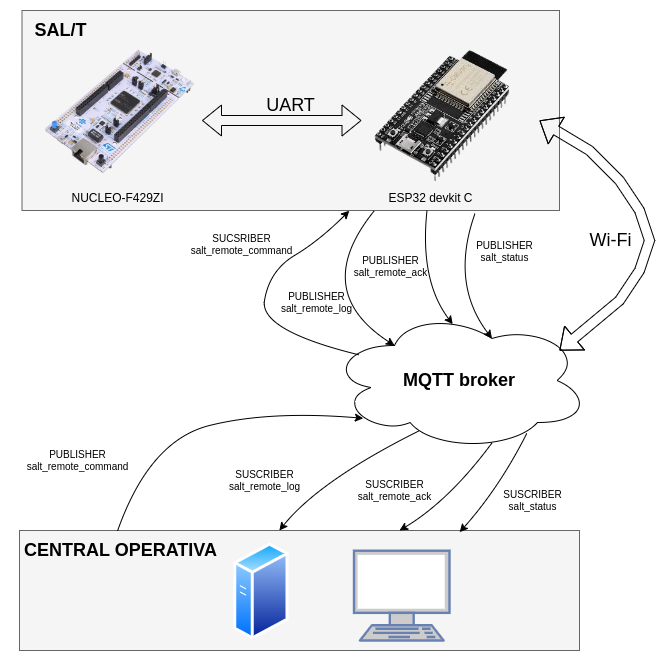
\includegraphics[width = \linewidth]{img/mqtt_bloques.png}    
    \caption{Diagrama de la comunicación entre el SAL/T y la central operativa}
    \label{fig:mqtt_bloque}
\end{figure}    




El \textit{topic} salt\_remote\_status se utiliza para que el SAL/T reporte su estado de manera periódica independientemente de los cambios que puedan ocurrir en el sistema. Por defecto, se reporta el estado general del sistema cada 5 segundos, siendo este tiempo un parámetro configurable del sistema. En este mensaje, se reporta el modo que esté activo en el SAL/T. El \textit{topic} salt\_remote\_log se utiliza para transmitir todos los cambios de estado del sistema y permitir guardar un registro de eventos en la central operativa en tiempo real. \\


Los \textit{topics} salt\_remote\_commands y salt\_remote\_ack se utilizan para el envío de comandos y confirmación de recepción entre la central operativa y el SAL/T. Los comandos enviados tienen una estructura de ID|COMANDO:PARÁMETROS que permite luego al sistema separar los distintos datos. De recibir y procesar correctamente el comando, el SAL/T va a responder por el \textit{topic} salt\_remote\_ack un mensaje con el formato ACK:ID utilizando el mismo ID recibido en el comando para confirmarle a la central operativa la recepción y ejecución del comando enviado. Los comandos que modifican el estado del SAL/T de manera continua tienen un tiempo de validez configurable, por defecto de 10 segundos, que una vez transcurrido son considerados inválidos. \\ 



A continuación se detallan los distintos comandos aceptados por el SAL/T y una breve explicación del comportamiento del sistema al recibirlos. 

\begin{itemize}
    \item \textbf{AISLADO\_TOTAL}: este comando fuerza el estado del SAL/T al modo aislado total donde todos los SIS son aislados y se liberan las señales de CT y FE. 
    
    \item \textbf{PARADA\_TOTAL}: este comando fuerza la activación de las señales de CT y FE del SAL/T llevando la formación a un estado de detención forzosa. 
    
    \item \textbf{COCHE\_DERIVA}: este comando fuerza la activación de la señal de corte de tracción, pero libera la señal de freno de emergencia aislando cualquier SIS que pueda estar activando la señal. 
    
    \item \textbf{INTERMITENTE:int}: este comando recibe un comando numérico del 1 al 5 que indica el perfil intermitente que se debe activar. El SAL/T pasa a estado intermitente siguiendo los tiempos de aceleración, desaceleración y freno configurados para el perfil seleccionado. 

    \item \textbf{CANCEL}: este comando cancela cualquier otro comando que esté vigente en el SAL/T. 
    
    \item \textbf{REPORT\_STATUS\_PERIOD\_CONFIG:int}: el parámetro corresponde a la cantidad de segundos que se desea configurar como período de transmisión de reporte de estado del SAL/T. Por defecto son 5 segundos pero se acepta la modificación en un rango de 1 a 60s. 
    
    \item \textbf{COMMAND\_VALIDITY\_CONFIG:int}: el parámetro corresponde a la cantidad de segundos que se desea configurar como tiempo de validez de un comando remoto activo. Por defecto son 10 segundos, pero se acepta la modificación en un rango de 1 a 60s. 
    
    \item \textbf{SPEED\_CONFIG:int,int,int,int,int}: se configura uno de los perfiles de velocidades que controlan la formación en el modo aislado limitado. El primer parámetro corresponde al perfil a configurar (valor entre 0 y 3 que corresponde a la zona de circulación 1, 2 y 3 y cuando no hay referencia de ubicación), luego los otros 4 parámetros corresponden a la velocidad límite para desacelerar, la velocidad límite para volver a acelerar en caso de activación del CT, la velocidad límite para aplicar el freno de emergencia y el tiempo mínimo de frenado una vez superado el umbral anterior. 
    
    \item \textbf{INTERMITENTE\_CONFIG:int,int,int,int,int}: se configura uno de los perfiles que controla la formación en modo intermitente. El primer parámetro corresponde al perfil a configurar (valor entre 1 y 5), luego los otros 4 parámetros corresponden el tiempo de aceleración por ciclo, el tiempo de desaceleración por ciclo, la cantidad de ciclos antes de aplicar el freno, y el tiempo de frenado luego de transcurridos los ciclos configurados. 
    
    \item \textbf{DOWNLOAD\_LOGS}: este comando permite extraer toda la información de registro de eventos que tiene almacenado el SAL/T internamente. Se transiten todos los eventos registrados a través del canal de logueo con la marca de tiempo correspondiente y un mensaje de inicio y de final de reporte para entender el contexto en el que se transmiten registros de eventos viejos. 
    
    \item \textbf{DATETIME:dd/MM/AAAA hh:mm:ss}: este comando no es enviado por la central operativa sino que es obtenido directamente por el ESP32 cada 10 segundos y enviado al MCU para que pueda sincronizar su fecha y hora con el informado por un servidor. 


\end{itemize}
